\documentclass[a4paper]{article}
\usepackage[utf8]{inputenc}
\usepackage[english]{babel}

\usepackage{amsmath}
\usepackage{amsfonts}
\usepackage{amssymb}
\usepackage{graphicx}
\usepackage{fancyhdr}
\usepackage{moreverb}
\usepackage{listings}
\usepackage{courier}
\usepackage{qtree}
\usepackage[normalem]{ulem}
\usepackage{color}
\usepackage{comment}
\usepackage{float}
\usepackage{enumitem}
\usepackage{etoolbox}

\newcommand{\setR}{\mathbb{R}}
\newcommand{\setZ}{\mathbb{Z}}
\newcommand{\setN}{\mathbb{N}}
\newcommand{\setF}{\mathbb{F}}
\newcommand{\lra}{\leftrightarrow}
\newcommand{\Lra}{\Leftrightarrow}
\newcommand{\ra}{\rightarrow}
\newcommand{\Ra}{\Rightarrow}
\newcommand{\tbf}[1]{\textbf{#1}}
\newcommand{\tit}[1]{\textit{#1}}
\newcommand{\tsc}[1]{\textsc{#1}}
\newcommand{\tsf}[1]{\textsf{#1}}
\newcommand{\tsl}[1]{\textsl{#1}}
\newcommand{\ttt}[1]{\texttt{#1}}
\newcommand{\subsubsubsection}[1]{\tbf{#1}\\}
\newcommand{\makeline}[1]{\noindent\makebox[\linewidth]{\rule{#1}{0.5pt}}}

\makeatletter
\pretocmd{\section}{\addtocontents{toc}{\protect\addvspace{1\p@}}}{}{}
\pretocmd{\subsection}{\addtocontents{toc}{\protect\addvspace{0\p@}}}{}{}

\lstset{	numbers=left,
		numberstyle=\footnotesize\ttfamily,
		numbersep=8pt,
		frame = single,
		basicstyle=\ttfamily,
		keywordstyle=\bfseries,
		commentstyle=\color{green},
		showstringspaces=false,
		morekeywords={include, printf, int, if, else, sizeof, void}
		}

\renewcommand{\headrulewidth}{0pt}

\title{Assisting Fuzzing with Concolic Execution}
\author{Søren Lund Jensen}
\begin{document}

\maketitle %TODO ændr til en flottere forside

\tableofcontents

\newpage
\section{Abstract}
\label{sec:Abstract}

\newpage
\section{Introduction and concept}
\label{sec:Intro}
An ever-present danger in today's society is memory corruption vulnerabilities in software, be they use of uninitialized memory, using dangling null-pointers, buffer overflow, memory leaks, or a fifth, sixth- or seventh vulnerabilities. An attacker could, did he know of these vulnerabilities, exploit them in order to access confidential informations, create DOS-attacks or other and as computer processing and connecting continues to be on the rise, playing a major role in present day, patching these vulnerabilities has to be a priority. This, of course, cannot be done without first discovering said bugs. 

Memory corruption bugs are often-case virtually untraceable, as only specific input combinations may trigger them, or the fact that they may appear under very unusual conditions, which makes it very hard to discover, or in some cases, even reproduce them. Add thereto, the fact, that the memory corruption's effect may manifest itself far away from its source, it can also be hard to even correlate these two, once a bug has been discovered.

A variety of tools exists, with the purpose of bug-discovery, but as the bugs are often very specific, and/or wide-spread, creating a silver bullet is hard, if not impossible. Many vulnerabilities are discovered manually, however, this solution is not scalable, as software applications generally increase in size and complexity. A handful of tools exist, including fuzzers and symbolic execution engines. These do, however have, in the worst cases, deal-breaking flaws, working against them, and their usefulness.

In late 2015, early 2016, The Defence Advanced Research Projects Agency (DARPA) hosted the 2016 Cyber Grand Challenge, with the theme of promoting and advancing automated computer security techniques, ranging from bug-detection to bug-squashing to hacking - all without interference from the teams who've created the software. Among the three teams, qualified for the final event, taking place August 2016 was Team Shellphish, who had created the Driller project: an extended version of American Fuzzy Lop, augmented by the concolic execution-engine, known as angr.

The idea behind this technology is to, through combining AFL with angr, mitigate as many of each of their respective drawbacks, while simultaneously utilizing many of their advantages - even create new symbiotic advantages.
\subsection{Problem statement}
\label{sec:problem}
Does Driller display a significant difference, in terms of running time and bugs/ vulnerabilities found, when compared to "regular" fuzzing, or is the technology?

Alternatively, is Driller suffering from being too narrowly engineered, as to better fit the kind of test-binaries given by DARPA, and so non-usable in real day intrusion-combating?
\newpage
\section{Team Shellphish}
\label{sec:Shellphish}
%TODO 1: Skriv section. 2: tænkt måske lidt som en pre-acknowledgement
\section{American Fuzzy Lop}
\label{sec:AFL}
This program works by feeding random input to a program, at a very high rate, some of which will hit specific vulnerabilities in said input-program. Every input fed is logged, and upon vulnerability-hit, AFL logs the input-ID. Hereafter information about where the vulnerability occurred, and which input triggered it is gatherable, based on input ID.

An advantage, as well as a drawback of most fuzzers, hereunder AFL is its execution method, which is to be as non-invasive as possible, as to prioritize speed before complexity handling. This means that AFL does not analyse a fuzzed application, but instead directly executing the application with random input, which is immensely faster than mutating qualified input variables, based on an application analysis.
\subsection{Features of AFL}
\label{sec:FeaturesAFL}
AFL implements a variety of features, to enhance its efficiency. In this section, I will list some of the key features, offered.\\
\subsubsubsection{Genetic Fuzzing}
When stating that the AFL fuzzing engine relies on executing applications with inputs at absolute random, one is not totally correct. This is due to the technique known as 'Genetic Fuzzing'. Genetic fuzzing means that the engine generates - \tit{unique} - inputs at total random. Simplified, this means that the current input, that AFL is generating cannot be the same as a previously generated input.\\
\subsubsubsection{Stable Transition Tracking}
AFL views the union of source and destination as a tuple of it's destination blocks. These tuples are prioritised, meaning that the tuples that cause the most different execution, compared to previous executions, are chosen first for future input generation.\\
\subsubsubsection{Loop Bucketization}
For a symbolic execution engines and fuzzers alike, loops are complicated to handle, as looping potentially offers an added layer of complexity. The AFL fuzzer makes the following contortions, in order to avoid looping's added complexity, and path space requirements:
When AFL detects that a triggered path contains a loop, it logs the executed loop iterations and compares this with previous inputs. The paths are grouped, based on the amount of iterations, and hereafter only \tit{one} path in a group is selected for further fuzzing. Using this the execution time of executing low loop-including paths is reduced to $O(log(N))$, as opposed to $O(N)$, if every single path should be discovered.\\
\subsubsubsection{De-randomization}
When AFL meets a random number, mutating one input value might not yield the same result, as mutating the same input value immediately after. Because of this, AFL features de-randomization, which allows for it to force randomized variables, to consistently use a specific seed, which in turn allows for consistent input/output-relations.
\newpage
\subsection{Limitations of AFL}
\label{sec:LimitsAFL}
Because of the union of the above techniques and its general nature, AFL is able to quickly discover a wide selection of general vulnerabilities, meaning vulnerabilities, that are triggered by some \tit{kind} of input. When vulnerability-triggers move past general input, and into the territory of general input AFL can potentially fall seriously behind.
\begin{lstlisting}[caption=A program that is difficult to fuzz, label=diffToFuzz, captionpos=b]
int main(void)
{
    int x;
    read(0, &x, sizeof(x));
    
    if (x == 0x12345678){
        vulnerability();
    }else{
         ...
    }
}
\end{lstlisting}
A generic example of this can be seen in Listing \ref{diffToFuzz}. This describes a program, that takes an input $x$ from a user. If, and only if, $x$ evaluates to $0x12345678$ the program will fail, as a vulnerability has been triggered, and as so, at each command, executed by the fuzzer, the frequency, and by extension, the chance of discovering the bug, is $1$ in $2^{32}$. Furthermore, as the AFL lacks the ability to produce new paths within this specific program lacks, it's instrumentation falls short, and AFL is reduced to randomly mutating non-instrumented input.
\section{Symbolic Execution}
\label{sec:SymEx}
Symbolic execution, or symbolic evaluation, is a way of program analysis, designed in order to determine the different ways said program can be executed, and which type of input causes it. Instead of executing actual values, to determine this, an interpreter assigns symbolic values to the input variables. The symbolic used to visualise how the program will execute, based on what \tit{kind} of input it will be fed.
\subsection{Features of Symbolic Execution}
\label{sec:FeaturesSymEx}
As symbolic execution relies on analysing input, instead of mindlessly executing input, it is able to detect specific inputs which, in this case, cause the application to crash. See Listing \ref{diffToFuzz} as an example. A symbolic execution engine will analyse it's functions, and generate the following tree:\\
\centerline{\Tree [.$\emptyset$ [. $x==0x12345678$ $\neg(x==0x12345678)$ ] ]}
\newpage
\noindent Another advantage of symbolic execution is the ability to invalidate sections input.
\begin{lstlisting}[caption=Example of Symbolic Execution, label=symExExample, captionpos=b]
int main(void)
{
    int x;
    read(0, &x, sizeof(x));
    
    if (x > 0x01){
        ...
    }else{
        ...
    }
    if x > 0x10){
        ...
    }else{
        ...
    }
}
\end{lstlisting}
In Listing \ref{symExExample} above, for example, the input $y$ is evaluated. A symbolic execution engine will analyse Listing \ref{symExExample}'s formulae, to find that $y$ will either assume a value greater than $0x01$ or not greater than $0x01$. Furthermore $y$ will either assume a value greater, or not greater than $0x10$, however greater than $0x10$ cannot occur, if $y$, at the same time was not greater than $0x01$. This will produce the following tree:\\
\centerline{
	\Tree [.$\emptyset$
			[.$y>0x01$ 
				[. $y>10$ 
				   $\neg(y>0x10)$
				]
			]
			[.$\neg(y>0x01)$
				[. \xout{$y>0x10$} 
				   $\neg(y>0x10)$ 
				]
			]
		]
}
Because of this trait, symbolic execution's relevance to the experiment is further heightened, as this allows for AFL to exclude certain value-ranges, when mutating input.
\subsection{Limitations of Symbolic Execution}
\label{sec:LimitsSymEx}
\subsubsubsection{Program-Dependent Efficiency}
The advantage of having a symbolic execution-engine analyse paths, as opposed to input, is not present in all programs. If some inputs take the same paths in a program, the difference in analysing the inputs instead of paths, is vanishingly small.\\
\subsubsubsection{Environment Interactions}
Often programs interact with their environment, such as executing system calls and/or receiving signals. This becomes a problem when these environment factors are not under the control of the symbolic execution tool, as the tool is not able to determine branching of a program, when it has insufficient data concerning input.\\
\subsubsubsection{Path Explosion}
The last, and possibly biggest drawback in symbolic execution engines is the path explosion problem. This problem is caused by a program that is containing loops, which causes the amount of path to grow exponentially. In theory the path amount can even become infinite, because of unbound loops. This problem is near-not-existing in small programs, however it often scales faster than the symbolically executed program scales, rendering symbolic execution virtually useless for testing medium to large applications.
\section{angr: The Concolic Execution Engine}
\label{sec:angr}
angr is a binary analysis framework, engineered modularly to be as versatile and composable as possible. Because of this, angr's use has potential to span wide, within the subject of binary analysis. Consider, for instance, just these few, but broad, uses of angr:
\begin{itemize}
	\item angr can be used as a dynamic symbolic execution engine, which combined with value set analysis, which allows to resolve bounds on symbolic variables.
	\item angr can be used as a static analysis engine, which also uses concolic tracing, in order to prove that detections are not false positives.
	\item angr can be used as a concolic tracer, along with a fuzzer, such as AFL, in order to allow for fully automatic bug discovery, such as what was done with Driller.
\end{itemize}
Driller would receive no benefit from invoking a regular symbolic execution engine, when stuck, as AFL cannot mutate input, based on symbolic values. Instead, using angr, an execution engine with the ability to mutate concrete values, based on the values found in the previous symbolic analysis-step.

angr, based on Mayhem \cite{Mayhem}, mutates concrete values via a four steps long algorithm. The steps can be broken down into the following:
\begin{itemize}
	\item[1] The input (i.e. binary code) is translated into Valgrind's VEX \cite{VEX} representation in order to determine the symbolic states of the binary code.
	\item[2] Symbolic values are set in place of all non-constant variables, such as user-defined input, randomized input, environment-dependant input, etc. Constant values are represented with the same concrete values, by which they are represented in the program.
	\item[3] The values are, by execution, given constraints set up by the binary environment, as well as the concrete values described in step 2.
	\item[4] When the program reaches a new path or state, input values, which drive the program to that state is generated, based on the constraints described step 2.
\end{itemize}
At any point after the algorithm has run, the gathered concrete values can be fed to the binary code, which will trigger the binary to produce an output similar to the one, that a corresponding symbolic value has generated.
\subsection{Diversity}
\label{sec:Diversityangr}
One of the design goals for angr has been to tailor it to be as diverse as possible. This was done, as angr was not only designed for its use in Driller, but was meant to be reusable, by team Shellphish, as well as any other security enthusiast out there. Because of this, angr was aimed towards support for ARM and MIPS processors, as well s 64-bit processors, instead of the 3-bit processors of yesteryear.

In the same spirit as the above mentioned cross-architecture support, angr also has to be able to support input, stemming from multiple platforms. This functionality is provided by the binary loader, called CLE, which is described in further detail in section \ref{sec:binaryLoader}.

Furthermore, when creating angr, team Shellphish did so, not only to further their odds in the DARPA CGC, but also to advance the bug-discovering community, and as a result of this, the tool is available as a fully editable open sourced program, completely free to use for any non-commercial use.
\subsection{The Binary Load Sub-Module}
\label{sec:binaryLoader}
When angr loads binaries into the application, it is handled by the binary load module, by the name of CLE. CLE is named, jokingly and recursively as an abbreviation for the sentence 'CLE Loads Everything'.

CLE is, as the point of departure, designed to work in the same way as GNU LD does with ELF binaries. This means that CLE does not necessarily load all the information in a binary, as some of this may be stripped or corrupted. When this happens, the ignored information is encompassed in a Project class. The rest of the information is stored in a Loader class, an in turn the CLE loader is representing a conglomerate of binaries, loaded by CLE, which, after being loaded, is mapped onto a single memory space. CLE has a subclass/ loader for each file type.

Currently, CLE offers support through its backends for PE, CGC, and both ordinary and core dump ELF files. Furthermore, CLE is able to load binaries with IDA, as well as loading files int flat address spaces. Which backend a binary file should use is auto-detectable for all, except the binaries, being loaded into flat images, which do need to be specified.
\section{Driller: Concolic Execution-Assisted Fuzzing}
\label{sec:Driller}
The core assumption, when team Shellphish designed Driller, was that 99+ \% of input could be divided into two categories: \tit{general} input, spanning over a broad pallet of values and \tit{specific} input, which is only able to take on a select few forms. Further chasing this assumption, the Driller approach emerges, which sees binaries as a collection of compartments. A representation of this can be seen in Figure \ref{Compartments} below:
\begin{figure}[H]
	\centering
	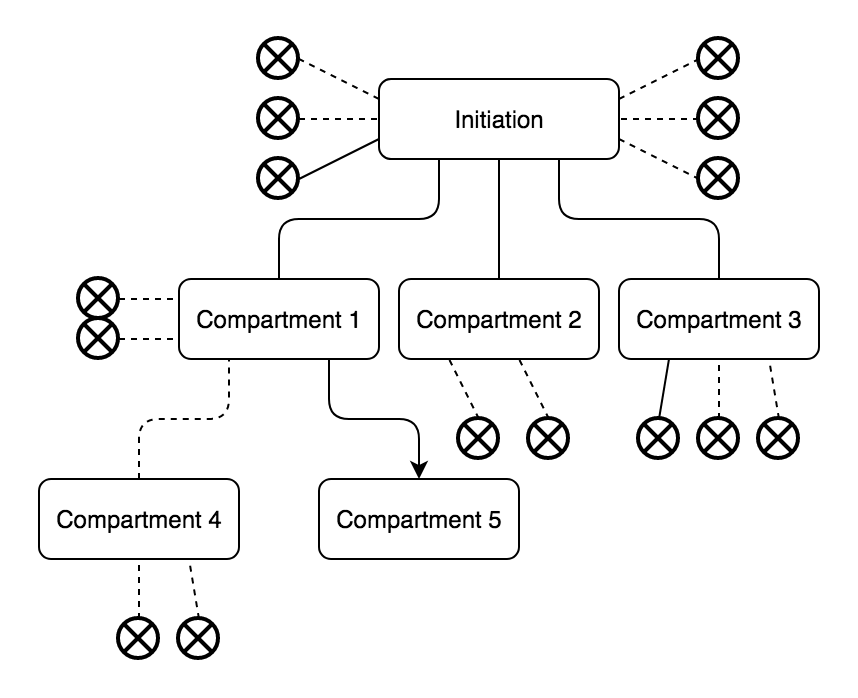
\includegraphics[width=0.5\textwidth]{Compartments}
	\caption{A graphic representation of binary compartments}
	\label{Compartments}
\end{figure}
\noindent
In Figure \ref{Compartments}, a path found by executing concolically is represented by a solid line, and a path found by means of fuzzing is represented by a dashed line. A bug is represented by $\otimes$. 

The vast majority of bugs found in Figure \ref{Compartments} is found by the fuzzing component, because of its wide-spread nature. A few bugs are still discovered by the concolic execution engine, but as this technique is very slow, the task of bug-discovery is primarily left to AFL.\\[0.1cm]
The task of discovering new components (i.e. paths) is primarily handled by angr. This doesn't mean that the fuzzer is unable to discover new paths, but the, sometimes very specific, input, required in order to move a program from one state to another is most efficiently handled by angr's concolic execution.
\subsection{Input Preconstraining}
\label{sec:preconstraining}
The union of the AFL fuzzer and angr's concolic execution, offers more advantages than just the union of the two's functionalities. The possibility of preconstraining input, by the concolic execution engine is introduced, as the two components are passing along information to on another, before doing their respective tasks. Consider Listing \ref{preconstraining} below:
\begin{lstlisting}[caption=A program in need of preconstraining,
label=preconstraining, captionpos=b]
int checker(bool *x, int limit)
{
    if (depth >= 100){
        return 0;
    }
    if (*x == 'TRUE'){
        counter = counter + checker(x + 1, limit + 1)
    } else{
        counter = counter + checker(x + 1, limit)
    }
    return counter;
} 
int main(void)
{
    bool x;
    int y;
    
    read(0, &x, sizeof(x));
    read(0, &y, sizeof(y));

    if (checker(x, 0 ) == 50){
        if (y == 0x12345678){
            vulnerability();
        }
    }	
    return 0;
}
\end{lstlisting}
This program would not be automatically de-buggable, by a fuzzer alone, neither a concolic execution engine, nor even a basic union of the two. A concolic execution engine would concede to the path explosion problem, when running the \ttt{checker} function, and a fuzzer would no be able to pass the check on line 23. Driller is not a basic union of these techniques, however, but a sophisticated collaboration. The information  gathered by AFL is passed along to angr, which is able to constrain its concolic execution, as to bypass the path explosion problem completely. What happens is as follows: AFL initially fuzzes the program, which leads it to, but not further than, line 23. From here, it quickly realizes that it is stuck, as the possibility of "guessing" the correct value for 
\ttt{y} is approximately $\frac{1}{2^{32}}$. Next, Driller invokes the concolic execution engine, and as this happens, Driller constrains the bytes in the symbolically executed input to match the input traced from AFL. Hereafter, only one branch is followed, as the tracing of AFL's data only will allow for this, and the path explosion problem has successfully been mitigated. When the concolic execution reaches line 23, however, it/Driller recognizes an alternate state transition, which has not previously been discovered by the fuzzing engine. At this point, as the path-exploding step has been overcome, Driller removes most of its constraints, not including the ones, leading through the line 23 check, where after \ttt{y} is constrained, forcing it to assume one of three unique concolic values:
\begin{itemize}[noitemsep]
	\item \ttt{y < 0x12345678}
	\item \ttt{y > 0x12345678}
	\item \ttt{y == 0x12345678}
\end{itemize}
At this point, Driller is quickly able to determine that two of these values will execute without any errors, but also that a third one, \ttt{y = 0x12345678} will result in a crash. 
\subsection{Re-randomization}
\label{sec:randomization}
Another issue, presented towards fuzzing, is the occurrence of random variables. Checks regarding these, have the ability to be as unfuzzable and difficult-to-hit as checks with normal specific input, but with the added challenge of being unstable, as it is virtually impossible to determine the value of a random variable, before utilizing it. Below, a listing, showcasing an example of this problem is presented.
\begin{lstlisting}[caption=A program featuring randomness,
label=randomness, captionpos=b]
int main(void)
{
    int x;
    int rand;
    
    read(0, &x, sizeof(x));
    rand = random();
    
    if (*x == *rand){
        vulnerability();
    }
}
\end{lstlisting}
Listing \ref{randomness} represents a small program, which is difficult to fuzz in the same way as Listing \ref{diffToFuzz}: regarding specific input. Furthermore, if a crash \tit{is} discovered here, a user have to manually observe the program output, in order to find what exactly crashed the program.

Luckily, this issue is easily handled by Driller. First of all, Driller's AFL component is very unqualified to handle the problem, and so forwards this to angr's concolic execution engine. The concolic execution engine breaks the input-variables into concolic values, as described in Section 5. Accordingly, this includes random variables, and as so, only three possibilities emerge:
\begin{itemize}[noitemsep]
	\item \ttt{x < rand}
	\item \ttt{x > rand}
	\item \ttt{x == rand}
\end{itemize}
Hereafter, angr quickly realizes that what triggers the found vulnerability isn't a specific value, assumed by the input variable \ttt{x}, but a specific \tit{relation} between \ttt{x} and \ttt{rand}. Driller is hereafter able to use this principle, as instances of random-variable-checks occurs in real non-test binaries and programs.
\subsection{The Algorithm}
\label{sec:TheAlgorithm}
\subsubsubsection{Input Test Cases}
Driller has no direct need for initial input test cases, and in such an instance, where non is provided, the initial fuzzing-step will work similarly to normal AFL-fuzzing. If initial test cases are provided, however, the initial fuzzing step can often times be sped up, as a tailored presence of these can guide AFL towards known compartments.\\
\subsubsubsection{Fuzzing}
When Driller is initiated, it begins by having AFL fuzz the initial compartment of the binary, which Driller has received as input. Driller discovers bugs in this compartment, by means of ordinary instrumented fuzzing, but will eventually reach a complex check, rendering AFL stuck, and therefore virtually useless.\\
\subsubsubsection{Concolic Execution}
At this point, Driller invokes its concolic execution engine angr. angr cross checks and pre-constrains the user-provided input with the input provided by AFL, in order to avoid path explosion, after which it calculates, via its constraint solving engine, which inputs would lead execution towards a new path, towards a new compartment. If AFL has discovered, and exhausted sub-compartments before the invoking of angr's concolic execution, these already-discovered paths would represent flows of execution into new compartments.\\
\subsubsubsection{Repeat and eventual halt}
When angr is eventually done with analysing the binary, having found new execution paths, the inputs, that trigger these are passed to the "testcases" folder. When AFL's fuzzing component is again invoked, the new input will be there for future mutation. From here, AFL's state transition tracking quickly determines that the new input will result in a radically different output, which is why they are chosen first for mutation. This simple back-and-forth between angr and AFL is what, when it comes down to it, Driller is made up of, and the ping-pong repeats itself until either an input resulting in a crash is discovered, or the execution is aborted by the user. 
\subsection{Additional Advantages of Driller}
\label{sec:DrillerAdditionalAdvantages}
The advantage of the combination of the technologies is vast. First of all the union of these two technologies are able to mitigate each of their biggest shortcomings (i.e. path explosion and specific input), by simply passing along the task, when a problem arises. Secondly, the information, gathered in angr can be utilized by AFL and vice versa. As such, angr does not only assist AFL in progressing deeper into the layers of the input binaries, but AFL further assists angr, with data, concerning executions, in order to avoid path explosion. Furthermore, angr's path explosion problem is additionally lowered, as angr does not necessarily have to analyse entire programs. Instead, because concolic execution with Driller only has the purpose to discover new paths, angr can analyse only a fraction of the program. This way, angr discovers only the compartments leading away from the current compartment, instead of every single state of the program at once, which will lead to a more smooth and uninterrupted fuzzing experience.

Because of these augmentations, Driller is able to work as not only an improved version of a concolic execution engine, but also like an improved version of AFL.
\section{Testing}
\label{sec:Testing}
Team Shellphish 
\subsection{Test Cases}
\label{sec:TestCases}
When testing Driller, Team Shellphish set two primary goals of achievement, as well as one secondary goal of documentation. The achievement goals were to prove, primarily, that Driller is able to expand on the code coverage, offered by fuzzers, instrumented as described in \ref{sec:FeaturesAFL}
\subsection{Results}
\label{sec:Results}
\subsubsection*{Comparable to non-instrumented Fuzzing}
\subsubsection*{Comparable to Symbolic Execution}
\section{Conclusion}
\label{sec:Conclusion}

\subsection{Discussion}
\label{sec:Discussion}

\subsection{Future Work}
\label{sec:FutureWork}
%Shellphish, der har lavet angr, har open-sourcet det, for at tillade videreudvikling - ergo er der OCEANER af 'future work'!
\section{Acknowledgements}
\label{sec:Acks}
%Shellphish
%Ellers bare kig på Acknowledgements i Drillerpapper
\begin{thebibliography}{9}
\bibitem{Driller}
	N. Stephens, J. Grosen, C. Salls, A. Dutcher, R. Wang, J. Corbetta, Y. Shoshitaishivili, C. Kruegel, G.  Vigna,
	Driller: Augmenting Fuzzing Through Selective Symbolic Execution,
	UC Santa Barbara,
	2016.
\bibitem{Mayhem} 
	S. K. Cha, T. Avgerinos, A. Rebert, and D. Brumley,
	Unleashing Mayhem on binary code,
	In Proceedings of the IEEE Symposium on Security and Privacy,
	2012.
\bibitem{VEX}
	N. Nethercote and J. Seward,
	Valgrind: a framework for heavyweight dynamic binary instrumentation, 
	In Proceedings of the ACM SIGPLAN Conference on Programming Language Design and Implementation (PLDI),
	Volume 42,
	pages 89–100, 
	ACM,
	2007.
\end{thebibliography}
\begin{comment}
Listinglabels
---------------
diffToFuzz
symExExample
randomness
preconstraining

Figurelabels
---------------
Compartments

Biblabels
---------------
Driller
Mayhem
VEX

Seclabels
---------------
sec:Abstract
sec:Intro
sec:Problem
sec:Shellphish
sec:AFL
sec:FeaturesAFL
sec:LimitsAFL
sec:SymEx
sec:FeaturesSymEx
sec:LimitsSymEx
sec:angr
sec:Diversityangr
sec:BinaryLoader
sec:Driller
sec:Preconstraining
sec:randomization
sec:TheAlgorithm
sec:DrillerAdditionalAdvantages
sec:Testing
sec:TestCases
sec:Results
sec:Conclusion
sec:FutureWork
sec:Acks
\end{comment}
\begin{comment}
idéer til mere rapport:
måske noget mere med intro
\end{comment}
\end{document}
